\documentclass[printbox]{BHCexam}
% \documentclass[openright,oneside]{ctexbook}	% 加[draft]选项可不显示图片本体,加快编译,全文完成后再删除

\biaoti{~$2019$~汤家凤考研线性代数强化}
\fubiaoti{邱日笔记}
\usepackage{ctex}
% \usepackage[heading=true]{ctex}

\usepackage{palatino}
\usepackage{siunitx}%输入度数符号需要的单位宏包
\usepackage{tikz}
% \usepackage[fntef]{ctexcap}
\usepackage{enumitem}
\usepackage{amsmath}
\usepackage{cases}
\usepackage[]{titlesec}
\usepackage{comment}%参看宏包说明
\usepackage{bbding}
\usepackage{mathdots}
\usepackage{cases}
% \usepackage{pmat}%分块矩阵的虚线,非miktex宏包,兼容性很好
% \iffalse \begin{pmat}[{.|}]
%     a_{11} & a_{12} & b_{11} \cr
%     a_{21} & a_{22} & b_{21} \cr\-
%     c_{11} & c_{12} & d_{11} \cr
%   \end{pmat}\fi
% \usepackage[center]{titlesec} %其中 center 可使标题居中,还可设为 raggedleft (居左,默认), raggedright (居右)。
% \titleformat{\chapter}{\centering\Huge\bfseries}{第\,\thechapter\,章}{1em}{}
%\CTEXsetup[name={第,章},number={\chinese{chapter}}]{chapter}

\usetikzlibrary{shapes.geometric, arrows}
\tikzstyle{startstop} = [rectangle, rounded corners, minimum width = 1cm, minimum height=0.5cm,text centered, draw = black]
\tikzstyle{io} = [trapezium, trapezium left angle=70, trapezium right angle=110, minimum width=0.5cm, minimum height=0.5cm, text centered, draw=black]
\tikzstyle{process} = [rectangle, minimum width=2cm, minimum height=0.5cm, text centered, draw=black]
\tikzstyle{decision} = [diamond, aspect = 3, text centered, draw=black]
% 箭头形式
\tikzstyle{arrow} = [->,>=latex]
\begin{document}
\AddEnumerateCounter{\chinese}{\chinese}{}

\printanswers % 我要打印答案

% \titleformat{\chapter}{\centering\Huge\bfseries}{第\,\thechapter\,章}{1em}{}
% \titleformat{\section}[block]{\centering\LARGE\bfseries}{第 \arabic{section} 章}{1em}{}
\titleformat{\section}[block]{\centering\LARGE\bfseries}{第 \chinese{section} 章}{1em}{}
\titleformat{\subsection}{\Large}{\chinese{subsection}. }{1em}{}
% \titleformat{\section}{\Large}{第\chinese{section}节 }{1em}{}
% \titleformat{\subsection}[block]{\Large\bfseries}{ \Roman{subsection}}{1em}{}
% \titleformat{\subsubsection}[block]{\large\bfseries}{\Roman{subsection}-\alph{subsubsection}}{1em}{}
% \titleformat{\paragraph}[block]{\normalsize\bfseries}{[\arabic{paragraph}]}{1em}{}


\maketitle  
% 暂时不搞标题节省时间

%\mininotice

% $\left(                 %左括号
% \begin{array}{ccc}   %该矩阵一共3列,每一列都居中放置
%   a11 & a12 & a13\\  %第一行元素      
%   a21 & a22 & a23\\  %第二行元素
% \end{array}
% \right)$      

\tableofcontents

\clearpage
% \part{部分标题}

% 垃圾


% \chapter{章标题}这一章我们介绍这些内容。

\section{行列式}
\subsection{defs}

\paragraph{1.} 逆序: $i,j \in N , if(i > j)  $
\paragraph{2.}  逆序数 \\
% \begin{enumerate}
  % \item 逆序: $i,j \in N , if(i > j)  $
  % \item 逆序数
  % \item 
  % \paragraph{}
D = $\begin{pmatrix} \begin{matrix} a_{ 11 } & ,... & a_{ 1n } \\ ... & ... & ... \\ a_{ n1 } & ... & a_{ nn } \end{matrix} \end{pmatrix}$=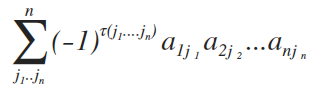
\includegraphics[scale=0.5]{assets/1-1.png}
  % $\begin{pmatrix} \begin{matrix} a_{ 11 } & a_{ 12 } & a_{ 13 } \\ a_{ 21 } & a_{ 22 } & a_{ 23 } \\ a_{ 31 } & a_{ 32 } & a_{ 33 } \end{matrix} \end{pmatrix}$ \\
$$=+a_{11} a_{22} a_{33} -a_{11} a_{23} a_{32} -a_{12} a_{21} a_{33} +a_{12} a_{23} a_{31}
+a_{13} a_{21} a_{32} -a_{13} a_{22} a_{31}
$$ 

  $\tau{(2\;5\;6\;4\; 1\; 2)} = 2+3+3+2$ 
  
    % +a_{11} 
  $\tau{(1 2 3)}=0,\tau{(132)}=1,\tau{(213)}=1,\tau{(231)}=2,\tau{(312)}=2,\tau{321}=3$

  \begin{numcases}{a_{11}}
   a_{22}  \qquad a_{33}\\
   a_{23}  \qquad a_{32}
  \end{numcases}
  \begin{numcases}{a_{12}}
    a_{21}  \qquad a_{33}\\
    a_{23}  \qquad a_{31}
   \end{numcases}
   \begin{numcases}{a_{13}}
    a_{21}  \qquad a_{32}\\
    a_{22}  \qquad a_{31}
   \end{numcases}

   \paragraph{3.}
   \begin{questions}
   \question 已知  ~$f(x)$~ = $\left(                 %左括号
   \begin{array}{ccc}   %该矩阵一共3列,每一列都居中放置
     2x-1 & x+2 & 3\\  %第一行元素      
     -1 & x+4 & 3-2x\\  %第二行元素
     5 & 3x+2 & x+2\\ 
   \end{array}
 \right)$                 %右括号
 ,求 ~$x^2$~系数.
%  \ifprintanswers
% Only if answers are printed
% \else
% Only if answers are not printed
% \fi
  
\begin{solution}
  \begin{numcases}{2x-1}
    x+4  \qquad x+2:  \qquad +(2x-1)(x+4)(x+2) \\
    3-2x  \qquad 3x+2: \qquad -(2x-1)(3-2x)(3x+2) 
   \end{numcases}
   \begin{numcases}{x+2}
      -1 \qquad x+2:  \qquad -(x+2)(x+4)(x+2) \\
     3-2x  \qquad 5 \qquad +(x+2)(3-2x)(5)
    \end{numcases}
    \begin{numcases}{3}
     -1  \qquad 3x+2  \qquad   \texttimes \\         %标准的叉
     x+4  \qquad 5 \qquad  \texttimes
    \end{numcases}
\end{solution}

\end{questions}  
%  \begin{solution}
%   \begin{parts}
%   \part $z=3+4\textbf{i}$
%   \part $\abs{z-w}\in[4,6]$
%   \end{parts}
%   \end{solution}
% https://en.wikibooks.org/wiki/LaTeX/Teacher%27s_Corner

% \Checkmark    %标准的勾
% \XSolid             %标准的叉
% \XSolidBrush
% \CheckmarkBold 
% \XSolidBold
  

\paragraph{4.}余子式与代数余子式\\

D=$\left(                 %左括号
\begin{array}{ccc}   %该矩阵一共3列,每一列都居中放置
  a_{11} & .. & a_{1n} \\  %第一行元素      
  .. & .. & ..\\  %第二行元素
  a_{n1} & .. & a_{nn}\\ 
\end{array}
\right)$                 %右括号

% ~$$~
% \substack{a\\\sim} 写在正上方
取~$a_{ij}~$. D去掉i行j列而成的n-1阶行列式,记~$M_{ij}-a_{ij}$~的余子式.\\
\centerline{~$A_{ij} \substack{\Delta \\=} (-1)^{i+j}M_{ij}$~}
\centerline{~$a_{ij}$~的代数余子式}





\subsection{特殊}
\paragraph{1.}
\ding{192}

$D_{2n}=\left|
\begin{array}{ccc}
  a_{11} &  & \\  %第一行元素   
   & \ddots & \\  %第一行元素     
   &  & a_{nn}\\  %第二行元素

\end{array}\right|$
$=\left|
\begin{array}{ccc}
  a_{11} &  & *\\  %第一行元素   
   & \ddots & \\  %第一行元素     
   &  & a_{nn}\\  %第二行元素
\end{array}\right|$ 
$=\left|
\begin{array}{ccc}
  a_{11} &  & \\  %第一行元素   
   & \ddots & \\  %第一行元素     
  * &  & a_{nn}\\  %第二行元素
\end{array}\right|$ 

\ding{193}
$\left|
\begin{array}{ccc}
   &  & l_1 \\  %第一行元素   
   & \iddots & \\  %第一行元素     
   l_n &  & \\  %第二行元素
  \end{array}\right|$ 
$=a_{11}...a_{nn}=(-1)^{\frac{n(n-1)}{2}}l_1...l_n$



$\tau(n\;...\;2\;1)=n-1+...+2+1$


%%%%%%%%%%%%%%%%%%%%%%%%%%%%%%%%%%%%%%%%邱日笔记第1页结束
\paragraph{2.}
$V_n{\substack{\Delta\\=}}\left|\begin{array}{cccc}
   1&  &1 & ... & 1\\  %第一行元素  
  a_{1} & a_{2} &... & a_{n}\\  %第一行元素   
...\\
  {a_1}^{n-1} &  {a_2}^{n-1}& &{a_n}^{n-1}\\  %第二行元素
\end{array}\right|$ 
$=\prod_{1\leq j < i \leq n } (a_i - a_j)$

$V_4=(a_4-a_1)(a_4-a_2)(a_4-a_3)(a_3-a_2)(a_2-a_1)$

Note: $V_n \neq 0 \Longleftrightarrow a_1...a_n$两两不等

\paragraph{3.}
\ding{192}
$=\left|
\begin{array}{cc}
  A &   \\  %第一行元素       
   &   B\\  %第二行元素
\end{array}\right|$ 
$=\left|
\begin{array}{cc}
  A &  C \\  %第一行元素       
  O &   B\\  %第二行元素
\end{array}\right|$ 
$=\left|
\begin{array}{cc}
  A &  O \\  %第一行元素       
  D &   B\\  %第二行元素
\end{array}\right|$
=~$|A|*|B|$~

\ding{193}
A,B为m n阶阵

$\left|
\begin{array}{cc}
   &A   \\  %第一行元素       
  B &   \\  %第二行元素
\end{array}\right|$ 
$=(-1)^{mn}\left|
\begin{array}{cc}
  B &   \\  %第一行元素       
   & A  \\  %第二行元素
\end{array}\right|$ 
$=(-1)^{mn}$
~$|A|*|B|$~
% $=(-1)^{mn}||$
% $=\prod_{i=1}^{n}$

\subsection{计算性质}
\begin{equation} 
\begin{cases} {}
  D \Longrightarrow $$
  \left(\begin{array}{ccc}

    \cdots   & \cdots &\cdots \\
                 & \ddots & \vdots \\
  % \multicolumn{2}{c}{\raisebox{1.3ex}[0pt]{\Huge0}}
                  &        &\vdots
  \end{array}\right)
  $$ \text{或}$$
  \left(\begin{array}{ccc}

    \ddots    &  &\\
    \vdots           & \ddots &  \\
  % \multicolumn{2}{c}{\raisebox{1.3ex}[0pt]{\Huge0}}
  \cdots            &    \cdots     &\cdots
  \end{array}\right)
  $$ \\
\text{降阶}
 \end{cases}
\end{equation}

% $$
%   \left(\begin{array}{cccc}
%   a_{11} & a_{12} & \cdots & a_{1n} \\
%          &a_{22}  & \cdots &a_{2n}  \\
%          &        & \ddots & \vdots \\
%   \multicolumn{2}{c}{\raisebox{1.3ex}[0pt]{\Huge0}}
%                   &        &a_{nn}
%   \end{array}\right)
%   $$ 

\paragraph{一.}
$D \Longrightarrow$ 
$\left(\begin{array}{ccc}
  \cdots   & \cdots &\cdots \\
               & \ddots & \vdots \\
% \multicolumn{2}{c}{\raisebox{1.3ex}[0pt]{\Huge0}}
                &        &\vdots
\end{array}\right)$
 或
 $
\left(\begin{array}{ccc}
  \ddots    &  &\\
  \vdots           & \ddots &  \\
% \multicolumn{2}{c}{\raisebox{1.3ex}[0pt]{\Huge0}}
\cdots            &    \cdots     &\cdots
\end{array}\right)$

\begin{questions}
\question \text{\bf{[例2]}}
$D=\left|
\begin{array}{ccc}
  a+b & b+c & c+a \\  %第一行元素   
  a_1+b_1& b_1+c_1 & c_1+a_1\\  %第一行元素     
  a2+b_2 & b_2+c_2  & c_2+a_2\\  %第二行元素
\end{array}\right|$.
$D=?$
% \end{questions}

\begin{solution}
  $D=\left|
\begin{array}{ccc}
  a+b & b+c & c+a \\  %第一行元素   
  a_1+b_1& b_1+c_1 & c_1+a_1\\  %第一行元素     
  a2+b_2 & b_2+c_2  & c_2+a_2\\  %第二行元素
\end{array}\right|$
$=\left|
\begin{array}{ccc}
  a & b+c & c+a \\  %第一行元素   
  a_1& b_1+c_1 & c_1+a_1\\  %第一行元素     
  a2 & b_2+c_2  & c_2+a_2\\  %第二行元素
\end{array}\right|$
$+\left|
\begin{array}{ccc}
  b & b+c & c+a \\  %第一行元素   
  b_1& b_1+c_1 & c_1+a_1\\  %第一行元素     
  b_2 & b_2+c_2  & c_2+a_2\\  %第二行元素
\end{array}\right|$

$=\left|
\begin{array}{ccc}
  a & b+c & c \\  %第一行元素   
  a_1& b_1+c_1 & c_1\\  %第一行元素     
  a2 & b_2+c_2  & c_2\\  %第二行元素
\end{array}\right|$
$+\left|
\begin{array}{ccc}
  b & c & c+a \\  %第一行元素   
  b_1& c_1 & c_1+a_1\\  %第一行元素     
  b_2 & c_2  & c_2+a_2\\  %第二行元素
\end{array}\right|$

$=\left|
\begin{array}{ccc}
  a & b & c \\  %第一行元素   
  a_1& b_1 & c_1\\  %第一行元素     
  a2 & b_2  & c_2\\  %第二行元素
\end{array}\right|$
$+\left|
\begin{array}{ccc}
  b & c & a \\  %第一行元素   
  b_1& c_1 & a_1\\  %第一行元素     
  b_2 & c_2  & a_2\\  %第二行元素
\end{array}\right|$

$=2\left|
\begin{array}{ccc}
  a & b & c \\  %第一行元素   
  a_1& b_1 & c_1\\  %第一行元素     
  a2 & b_2  & c_2\\  %第二行元素
\end{array}\right|$
\end{solution}





%%%%%%%例3
% \begin{questions}
\question \text{\bf{[例3]}}~$A=(\alpha_1,\alpha_2,\gamma_1),B=(\alpha_1,\alpha_2,\gamma_2)
$~.~$|A|=3,|B|=2,求|A+2B|$~.

\begin{solution}
  ~$A+2B=(\alpha_1,\alpha_2,\gamma_1)+(\alpha_1,\alpha_2,\gamma_2)=
  (3\alpha_1,3\alpha_2,\gamma_1+2\gamma_2)$~.

  ~$|A+2B|=|3\alpha_1,3\alpha_2,\gamma_1+2\gamma_2|=9|\alpha_1,\alpha_2,\gamma_1+2\gamma_2|\\
  =9(|\alpha_1,\alpha_2,\gamma_1+ 2|\alpha_1,\alpha_2,\gamma_2|)\\
  =9(|A|+2|B|)=63
  $~
\end{solution}

\question \text{\bf{[例4]}} $D=\left|
\begin{array}{ccc}
  3&1&1\\
  1&3&1\\
  1&1&3\\
\end{array}\right|$.
$D=?$
\end{questions}
\begin{solution}
  $D=5\left|
\begin{array}{ccc}
  1&1&1\\
  \underline{1}&3&1\\
  \underline{1}&1&3\\
\end{array}\right|$
$=5\left|
\begin{array}{ccc}
  1&1&1\\
  0&2&0\\
  0&0&2\\
\end{array}\right|=20$
\end{solution}

\paragraph{二.}降阶1
\begin{questions}
\question
$D=\left|
\begin{array}{ccc}
  1&-1&2\\
  2&0&11\\
  3&1&4\\
\end{array}\right|,\text{求}D$
\end{questions}
\begin{solution}

 法一: $D=\left|
\begin{array}{ccc}
  1&-1&2\\
  0&2&7\\
  0&\boxed{4}&-2\\
\end{array}\right|,$
$=\left|
\begin{array}{ccc}
  1&-1&2\\
  0&2&7\\
  0&0&-16=-32\\
\end{array}\right|,$

法二: $D=1*(-11)+(-1)*25+2*2=-11-25-4=-32$

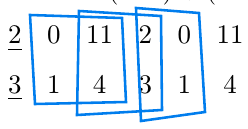
\includegraphics[scale=0.5]{assets/1-2.png}

% $D=\left|
% \begin{array}{cccccc}
%   \sout{2}&0&11&2&0&11\\
%  \sout{3}&1&4&3&1&4\\
% \end{array}\right|,$

$\begin{cases}{}
  a_{11}=1  \qquad M_{11}-11  \qquad A_{11}=-11\\
  a_{12}=1  \qquad M_{12}-25  \qquad A_{12}=-25\\
  a_{13}=2  \qquad M_{11}-2  \qquad A_{13}=2
 \end{cases}
 \begin{cases}{}
  a_{21}=2  \qquad M_{21}=-6  \qquad A_{21}=6\\
  a_{22}=0  \qquad M_{22}=-2  \qquad A_{22}=-2\\
  a_{23}=11  \qquad M_{21}=4  \qquad A_{23}=4
 \end{cases}\\
 \begin{cases}{}
  a_{31}=3  \qquad M_{31}=-11  \qquad A_{31}=-11\\
  a_{32}=1  \qquad M_{32}=-7  \qquad A_{32}=-7\\
  a_{33}=4  \qquad M_{31}=2  \qquad A_{33}=2
 \end{cases}
 \begin{cases}{}
  -11-25+4=-32\\
  12+0-44=-32\\
 -33-7+8=-32
 \end{cases}
 \begin{cases}{}
 6+20+8=0\\
 -11+7+4=0
\end{cases}$
\end{solution}

\paragraph{三.}降阶2

1.$\begin{cases}{}
a_{i1}A_{i1}+a_{i2}A_{i2}+...+a_{in}A_{in}=D\\
a_{1j}A_{1j}+a_{2j}A_{2j}+...+a_{nj}A_{nj}=D
 \end{cases}\\
 (i,j=1,2,...,n)$

2.$a_{i1}A_{i1}+a_{i2}A_{i2}+...+a_{in}A_{in}=0\\
 (i \neq j)$

Notes:
\ding{192}行列式中出现$A_{ij},A^{*}$

$A^{*}=\left(                 %左括号
\begin{array}{ccc}   %该矩阵一共3列,每一列都居中放置
   A_{11}& .. & A_{1n} \\  %第一行元素      
  .. & .. & ..\\  %第二行元素
  A_{n1} & .. & A_{nn}\\ 
\end{array}
\right)$                 %右括号

$ \begin{cases}{}
  |A^{*}|=|A|^{n-1}\\
  a_{i1}A_{i1}+...+a_{in}A_{in}=D
 \end{cases}$


\begin{questions}
  \question
$D=\left(
\begin{array}{ccc}
  a&a&a\\
  &*&
\end{array}\right)_{3*3}.(a>0)\\
A_{ij}=a_{ij},a=\mtk{}$

\begin{solution}
  $A^{*}=\left(                 %左括号
\begin{array}{ccc}   %该矩阵一共3列,每一列都居中放置
   A_{11}& A_{21} & A_{31} \\  %第一行元素      
   A_{12}& A_{22} & A_{32} \\  %第一行元素  
   A_{13}& A_{23} & A_{33} \\  %第一行元素  
\end{array}
\right)$
$=A^{T}\\
|A^{*}|=|A^{T}| \Longrightarrow |A|^2 =|A|\\
|A|=0\text{或}|A|=1\\
|A|=a_{11}A_{11}+a_{12}A_{12}+a_{13}A_{13}=3a^2>0 \Longrightarrow a=\frac{1}{\sqrt{3}}$ 
\end{solution}

\question
$A^{*}=\left(                 %左括号
\begin{array}{ccc}   %该矩阵一共3列,每一列都居中放置
  2   & a_{12} & a_{13} \\  %第一行元素      
   & * &  \\  %第一行元素  
   & * &  \\  %第一行元素  
\end{array}
\right)_{3*3}$
$,A_{ij}+3a_{ij}=0,|A|=?$

\begin{solution}
  $,A_{*}=-3a^{T}\\
  |A_{*}|=|-3a^{T}| \Longrightarrow |A|^2 = -27|A| \Longleftarrow |A|=0\text{或}A=-27\\
  |A|=-3(a_{11}^2+a_{12}^2+a_{13}^<0)\\
  \therefore |A|=-27
  $
\end{solution}

\ding{193}稀疏行列式用降阶计算

\question
$A^{*}=\left|                 %左括号
\begin{array}{cccc}   %该矩阵一共3列,每一列都居中放置
a &-1&0&0\\
2a & a &-1&0\\
0&2a&a&-1\\
0&0&2a&a
\end{array}
\right|$                 %右括号

\end{questions}
\begin{solution}
  $D=aA_{11}+(-1)A_{12}\\
  =aM_{11}+M_{12}\\$
$=a\left|                 %左括号
  \begin{array}{ccc}   %该矩阵一共3列,每一列都居中放置
  a &-1&0\\
  2a&a&-1\\
0&2a&a\\
  \end{array}
  \right|$                 %右括号
$+\left|                 %左括号
  \begin{array}{ccc}   %该矩阵一共3列,每一列都居中放置
  \boxed{2a} &-1&0\\
  0&a&-1\\
0&2a&a\\
  \end{array}
  \right|$                 %右括号
$=a[aA{11}+(-1)A_{11}+2a(a^2+2a)]$\\
$= a^2M_{11}+aM_{12}+2a^{3}+4a^2$

\end{solution} 

\subsection{应用}
(*)式:$\begin{cases}{}
  a_{11}x_1+...+a_{1n}x_{n}=0\\
  a_{n1}A_{1j}+...+a_{nn}x_{n}=0
   \end{cases}\\$

   (**)式:$\begin{cases}{}
    a_{11}x_1+...+a_{1n}x_{n}=b1\\
    a_{n1}A_{1j}+...+a_{nn}x_{n}=bn
     \end{cases}\\$


Th1:对(*):\\
\ding{192}~$D \neq 0\Longleftrightarrow r(A)=n \Longleftrightarrow
(*)$~只有零解\\
\ding{193}~$D = 0\Longleftrightarrow r(A)<n \Longleftrightarrow
(*)$~除零解外有非零解(有无数解)\\
Th2:对(**):\\
\ding{192}~$D \neq 0\Longleftrightarrow r(A)=r(\widetilde{A})=n \Longleftrightarrow
(**)$~有唯一解且$x_i=\frac{D_i}{D}(1\leq i \leq n );$\\
\ding{193}~$D=0\Longleftrightarrow r(A)<n $

$\begin{cases}{}
  r(A)=r(\widetilde{A})<n \Longleftrightarrow \text{(**)有无数解}\\
  r(A)<r(\widetilde{A})\Longleftrightarrow \text{(**)无解}
   \end{cases}\\$



\section{矩阵(表格)}
\subsection{defs}
\paragraph{1.}
$A=\left(                 %左括号
\begin{array}{ccc}   %该矩阵一共3列,每一列都居中放置
  a_{11} & .. & a_{1n} \\  %第一行元素      
  .. & .. & ..\\  %第二行元素
  a_{m1} & .. & a_{mn}\\ 
\end{array}
\right)$                 %右括号
$\substack{\Delta \\=}{(a_{ij})}_{m*n}$\\

\ding{192}$A_{m*n}\;if\;m=n\quad $A为n阶方阵\\
\ding{193}$A=(a_{ij})_{m*n}\qquad if\;\forall a_{ij}=0,A=0$\\
\ding{194}$A=\left(                 %左括号
\begin{array}{ccc}   %该矩阵一共3列,每一列都居中放置
  a_{1} &  &  \\  %第一行元素      
  & \ddots & \\  %第二行元素
& & a_{n}\\ 
\end{array}
\right)$                 %右括号
对角矩阵\\
\ding{195}$A=\left(                 %左括号
\begin{array}{ccc}   %该矩阵一共3列,每一列都居中放置
  k &  &  \\  %第一行元素      
  & \ddots & \\  %第二行元素
& & k\\ 
\end{array}
\right)$                 %右括号
数量矩阵\\
\ding{196}$A=\left(                 %左括号
\begin{array}{ccc}   %该矩阵一共3列,每一列都居中放置
  a_{11} &  & a_{1n} \\  %第一行元素      
  & \cdots & \\  %第二行元素
a_{n1}& & a_{nn}\\ 
\end{array}
\right)$                 %右括号
$if\;\forall a_{ij}=a_{ji}$\qquad A称为对称矩阵\\
\ding{197}$A=\left(                 %左括号
\begin{array}{ccc}   %该矩阵一共3列,每一列都居中放置
  a_{11} &  & a_{1n} \\  %第一行元素      
  & \cdots & \\  %第二行元素
a_{n1}& & a_{nn}\\ 
\end{array}
\right)$                 %右括号
$if\;\forall A^{T}=E$\qquad A称为正交矩阵\\

\paragraph{2.}同型\\
$A_{m*n},B_{m*n},$称 $\widetilde{\text{同型}}$\\
$if\; \forall a_{ij}=b_{ij},$称$A=B$

\paragraph{3.}三则\\
\ding{192}$A \pm B$;\\
\ding{193}$kA$\\
\ding{194}$A_{m \times n} =
\left(                 %左括号
\begin{array}{ccc}   %该矩阵一共3列,每一列都居中放置
  a_{11} &  & a_{1n} \\  %第一行元素      
  & \cdots & \\  %第二行元素
a_{n1}& & a_{mn}\\ 
\end{array}
\right)$,                 %右括号
$B_{n \times s} =
\left(                 %左括号
\begin{array}{ccc}   %该矩阵一共3列,每一列都居中放置
  b_{11} &  & b_{1s} \\  %第一行元素      
  & \cdots & \\  %第二行元素
b_{n1}& & b_{ns}\\ 
\end{array}
\right)$   \\              %右括号

$A_{m \times \underline{n}}B_{\underline{n} \times s} $,合法看内标\\
型看外标.\\
$AB= C_{m \times s} =
\left(                 %左括号
\begin{array}{ccc}   %该矩阵一共3列,每一列都居中放置
  c_{11} &  & c_{1s} \\  %第一行元素      
  & \cdots & \\  %第二行元素
c_{m1}& & c_{ms}\\ 
\end{array}
\right)$   \\              %右括号

Notes:

\ding{192}
$\begin{cases}
  A \neq 0,B \neq 0, \nRightarrow AB \neq 0 \\
  A \neq 0, \nRightarrow  A^{*} \neq 0 \\
  AB \neq BA 
\end{cases} \\
$

\ding{193}\\
$f(x)= a_nx_n+...+a_1x+a_0, \qquad A_{m \times n }\\
f(A)\substack{\Delta \\=} a_nA_n+...+A_1x+A_0E
$\\因式分解

$\begin{cases}{}
  a_{11}x_1+...+a_{1n}x_{n}=0\\
  a_{m1}A_{1j}+...+a_{mn}x_{n}=0
   \end{cases}(*)\\$

$\begin{cases}{}
  a_{11}x_1+...+a_{1n}x_{n}=b_1\\
  a_{m1}A_{1j}+...+a_{mn}x_{n}=b_n
   \end{cases}(**)\\$

   $\left(                 %左括号
   \begin{array}{ccc}   %该矩阵一共3列,每一列都居中放置
     a_{11} & ... & a_{1n}\\  %第一行元素      
     a_{m1} & ... & a_{mn}\\ 
   \end{array}
 \right)$                 %右括号

 $X=\left(                 %左括号
 \begin{array}{c}   %该矩阵一共3列,每一列都居中放置
   x_{1} \\  %第一行元素 
   \vdots\\     
   x_{n} \\ 
 \end{array}
\right)$,                 %右括号
$b=\left(                 %左括号
\begin{array}{c}   %该矩阵一共3列,每一列都居中放置
  b_{1} \\  %第一行元素 
  \vdots\\     
  b_{n} \\ 
\end{array}
\right)$                 %右括号

$\begin{cases}{}
  AX=0,\qquad (*) \\
  AX=b,\qquad (**)
   \end{cases}\\$

   \paragraph{4.}伴随矩阵\\
   $A=\left(                 %左括号
   \begin{array}{ccc}   %该矩阵一共3列,每一列都居中放置
     a_{11} & ... & a_{1n}\\  %第一行元素      
     a_{m1} & ... & a_{mn}\\ 
   \end{array}
 \right)$                 %右括号
 $ \Longrightarrow  
|A|=\left|                 %左括号
\begin{array}{ccc}   %该矩阵一共3列,每一列都居中放置
  a_{11} & ... & a_{1n}\\  %第一行元素      
  a_{m1} & ... & a_{mn}\\ 
\end{array}
\right|$     
$ \forall a_{ij} \Longrightarrow M_{ij} \Longrightarrow A_{ij} \\
\Longrightarrow $
$A^*=\left(                 %左括号
\begin{array}{cccc}   %该矩阵一共3列,每一列都居中放置
  A_{11} & A_{21} & \cdots & A_{n1}\\  %第一行元素   
  A_{12} & A_{22} & \cdots & A_{n2}\\  %第一行元素
  \vdots & \vdots  & \cdots & \vdots \\  %第一行元素          
  A_{1n} & A_{2n} & \cdots & A_{nn}\\ 
\end{array}
\right)$ 称为A的伴随矩阵\\

Notes:\\
\ding{192}
$\begin{cases}
  |A^T|=|A| \\
  |kA|=k^n|A|\\
  |AB|=|A||B|\qquad(Laplace\;rule)\\
  |A^*=|A|^{n-1}\\
\end{cases}$
\ding{193}
$A|A|^*=A^*A=|A|E$

Q:矩阵的研究对象?\\
ax=b\qquad $\begin{cases}
  a \neq 0  \qquad \frac{1}{a} * a =1 \Longrightarrow x = \frac{b}{a} \\
  a = 0 \qquad (b =0 \text{无数解} \; or \; b \neq 0 \text{无解})
\end{cases}$
 
%  $

% $D_{2n}=\left|
% \begin{array}{cccccccccc}
% a& & & & & & & & &b\\
%  &a& & & & & & &b& \\
%  & & &\ddots& & &\iddots& & & \\
%  & & & &a&b& & & & \\
%  & & & &b&a& & & & \\
%  & & &\iddots& & &\ddots& & & \\
%  &b& & & & & & &a& \\
% b& & & & & & & & &a\\
% \end{array}\right|$
   
%    $\left(                 %左括号
%    \begin{array}{ccc}   %该矩阵一共3列,每一列都居中放置
%      a11 & a12 & a13\\  %第一行元素      
%      a21 & a22 & a23\\  %第二行元素
%    \end{array}
%  \right)$      
%  $\left(                 %左括号
%  \begin{array}{ccc}   %该矩阵一共3列,每一列都居中放置
%    a11 & a12 & a13\\  %第一行元素      
%    a21 & a22 & a23\\  %第二行元素
%  \end{array}
% \right)$      
  %  \begin{parts}
  %  \part 当~$a=1$~时,求曲线~$f(x)$~在~$x=1$~处的切线方程;
  %  \part 设函数~$h(x)=f(x)-g(x)$~,求函数~$h(x)$~的单调区间.
  %  \end{parts}

  
   


    % $$\begin{equation}       %开始数学环境
      $\left(                 %左括号
        \begin{array}{ccc}   %该矩阵一共3列,每一列都居中放置
          2x-1 & x+2 & 3\\  %第一行元素      
          -1 & x+4 & 3-2x\\  %第二行元素
          5 & 3x+2 & x+2\\ 
        \end{array}
      \right)$                 %右括号
% $\sum _{ j_{ 1 }..j_{ n } }^{ n }{ (-1)^{ \tau (j_{ 1 }....j_{ n }) } } a_{ 1 }_{ j }_{ _{ 1 } }a_{ 2 }_{ j }_{ _{ 2 } }...a_{ n }_{ j }_{ _{ n } }$


% \end{enumerate}


\paragraph{逆序}

\begin{enumerate}[label={\chinese*、},labelsep=0pt]

  \item defs


  \item 格式美观

\end{enumerate}



\section{节标题}这一节我们介绍这些内容

    \begin{numcases}{|x|=}
    x, & $x \geq 0$\\
    -x, &  $x < 0$
    \end{numcases}
    % $$\begin{equation}       %开始数学环境
      $\left(                 %左括号
        \begin{array}{ccc}   %该矩阵一共3列,每一列都居中放置
          a11 & a12 & a13\\  %第一行元素      
          a21 & a22 & a23\\  %第二行元素
        \end{array}
      \right)$                 %右括号
      % \end{equation}$$


\AddEnumerateCounter{\chinese}{\chinese}{}

\begin{enumerate}[label={\chinese*、},labelsep=0pt]

  \item 内容清晰


  \item 格式美观

\end{enumerate}
\subsection{逆序}


\subsection{小节标题}这一小节我们介绍这些内容。
\subsubsection{子节标题}这一子节我们介绍这些内容。
\paragraph{段标题}这一段我们介绍这些内容。
\subparagraph{小段标题}这一小段我们介绍这些内容。

\section{微分中值定理}

\subsection{费马极值定理}

\notice




\begin{questions}


%选择题
\xuanze

\question 已知椭圆~$\dfrac{x^2}{16}+\dfrac{y^2}{m}=1$~的一个焦点为~$F(3,0)$~,则~$m=$~\xx.
\onech{$3$}{$7$}{$9$}{$25$}
\question 下列函数中,既是奇函数又是定义域上的增函数的是\xx.
\onech{$y=2x+1$}{$y=e^x-e^{-x}$}{$y=\dfrac{-2}{x}$}{$y=x\sqrt{x}$}
\question 设等差数列~$\{a_n \}$~的前~$n$~项和为~$S_n$~,若~$S_3=18$~,则~$a_2$~\xx.
\onech{$7$}{$5$}{$6$}{$4$}
%\begin{minipage}[b]{0.6\linewidth}
\question 函数~$f(x)=A\sin (\omega x+\varphi)$($A,\omega,\varphi$~是常数,~$A>0,\omega >0$)~的部分图象如图所示,则函数~$f(x)$~的单调增区间可能为\xx.
\fourch{$\left[ -\dfrac{5\pi}{12},\dfrac{\pi}{12} \right]$}{$\left[ -\dfrac{\pi}{3},\dfrac{\pi}{6} \right]$}%
{$\left[ \dfrac{\pi}{12},\dfrac{7\pi}{12} \right]$}{$\left[ -\dfrac{\pi}{12},\dfrac{5\pi}{12} \right]$}
\vspace{-3.5cm}
\begin{center}
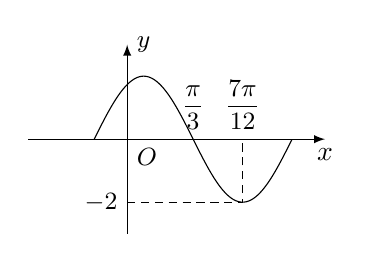
\begin{tikzpicture}[scale=0.8]
\coordinate[label=below right:\small $O$] (O) at(0,0);
\coordinate[label=above :\small $\dfrac{\pi}{3}$] (t1) at(pi/3,0);
\coordinate[label=above :\small $\dfrac{7\pi}{12}$] (t2) at(7*pi/12,0);
\draw[->,>=latex](-pi/2,0)--(pi,0)node[below](x) {$x$};
\draw[->,>=latex](0,-1.5)--(0,1.5)node[right](y) {\small $y$};
\draw [domain=-pi/6:5*pi/6,samples=1000] plot(\x,{sin((2*(\x)+pi/3) r)});
\draw[densely dashed](0,-1)--(7*pi/12,-1)--(7*pi/12,0);
\node[left](pi) at(0,-1) {\small $-2$};
\end{tikzpicture}
\end{center}
%\end{minipage}
%\hfill
%\begin{minipage}[b]{0.4\linewidth}
%\end{minipage}
\question 下列有关命题的说法正确的是\xx.
\fourch{命题“若~$x=y$~,则~$\sin x=\sin y$~”的逆否命题为真命题}{函数~$f(x)=\tan x$~的定义域为~$\{x\,|\,x\neq k\pi,k\in Z$~}
{命题“~$\exists x\in R$~使得~$x^2+x+1<0$~”的否定是:“~$\forall x\in R$~,均有~$x^2+x+1<0$~".}
{“$a=2$~”是“直线~$y=-ax+2$~与~$y=\dfrac{a}{x} x-1$~垂直”的必要不充分条件.}
\question 执行如图所示的程序框图,输出的$s$值为~\xx.
\twoch{$-3$}{$-\dfrac{1}{2}$}{$2$}{$\dfrac{1}{3}$}
\question 设函数~$y=x^3$~与~$y=\left(\dfrac{1}{2} \right)^{x-2}$~的图象的交点为~$(~x_0,y_0~)$~,则~$x_0$~所在的区间是\xx.
\twoch{$(0,1)$}{$(1,2)$}{$(2,3)$}{$(3,4)$}
\question 一个空间几何体的三视图如图,则该几何体的体积为\xx.

\twoch{$2\sqrt{3}$}{$2\sqrt{5}$}{$\dfrac{4\sqrt{3}}{3}$}{$\dfrac{5\sqrt{3}}{3}$}
\clearpage
\begin{figure*}[!htb] 
\begin{minipage}[t]{0.5\textwidth}%并排放两张图片,每张占页面的0.5,下同。  
\vspace{-1cm}
\centering  
% \includegraphics[scale=0.9]{liuchengtu.pdf}
\end{minipage}  
\begin{minipage}[t]{0.5\textwidth}  
\vspace{0cm}
\centering  
% \includegraphics[scale=0.9]{sanshitu.pdf}
\end{minipage}  
\end{figure*}
\vspace{-2cm}
%填空题
\tiankong
\question 已知向量~$\vec{a}=(3,1),\vec{b}=(1,3),\vec{c}=(k,7)$~,若~$(\vec{a}-\vec{c}) \parallel \vec{b}$~,则~$k=$~\mtk{}.
\question 等比数列~$\{a_n \}$~的公比~$q>0$~,已知~$a_2=1,a_{n+2}+a_{n+1}=6a_n$~,则~$\{a_n \}$~的前~$4$~项和~$S_4$~\mtk{}.
\question 设~$z=kx+y$~,其中实数~$x,y$~满足~$ \begin{cases}
x+y-2\geq 0,\\
x-2y+4\geq 0, \\
2x-y-4\leq 0,
\end{cases}$若~$z$~的最大值为~$12$~,则实数~$k=$~\mtk{}.
\question 设~$f(x)$~表示~$x+2$~与~$x^2+3x+2$~中的较大者,则~$f(x)$~的最小值为\mtk{}.
\question 设~$a\in R,f(x)=\cos (a\sin x-\cos x)+\sin ^2 x$~的定义域是~$\left[ \dfrac{\pi}{4},\dfrac{11}{24} \pi \right]~,f(\dfrac{\pi}{4})=\sqrt{3}$~.\\给出下列几个命题:\\
\ding{192}~$f(x)$~在~$x=\dfrac{\pi}{4}$~处取得最小值;\ding{193}~$\left[ \dfrac{5}{12} \pi,\dfrac{11}{24} \pi \right]$~是~$f(x)$~的一个单调递减区间;\\
\ding{194}~$f(x)$~的图象向左平移~$\dfrac{\pi}{12}$~个单位,将得到函数~$y=2\sin {2x}$~的图象;\\
\ding{195}使得~$f(x)$~取得最大值的点仅有一个~$x=\dfrac{\pi}{3}$~.\\
其中正确命题的序号是\mtk{}.(将你认为正确命题的序号都填上)
%解答题
\jianda
\question 在~$\triangle ABC$~中,角~$A,B,C$~的对边分别为~$a,b,c$~,已知~$A=\dfrac{\pi}{2}+C,\sin (A+C)=\dfrac{3}{5}$~.
\begin{parts}
\part 求~$\cos C$~的值;
\part 若~$a+c=3\sqrt{5}$~,求~$\triangle ABC$~的面积.
\end{parts}
\vspace{6cm}
\question 有甲乙两个班级进行数学考试,按照大于等于分为优秀,分以下为非优秀统计成绩后,得到如下的列联表.
\begin{center}
\begin{tabular}{|c|c|c|c|}
\hline
~~~~~~~{}~~~~~~~&~~~~~~~优秀~~~~~~~&~~~~~~~非优秀~~~~~~~&~~~~~~~总计~~~~~~~\\
\hline
~~~~~~~甲班~~~~~~~&~~~~~~~10~~~~~~~&~~~~~~~{}~~~~~~~&~~~~~~~{}~~~~~~~\\
\hline
~~~~~~~乙班~~~~~~~&~~~~~~~{}~~~~~~~&~~~~~~~30~~~~~~~&~~~~~~~{}~~~~~~~\\
\hline
~~~~~~~合计~~~~~~~&~~~~~~~{}~~~~~~~&~~~~~~~{}~~~~~~~&~~~~~~~105~~~~~~~\\
\hline
\end{tabular}
\end{center}
已知在全部~$105$~人中抽到随机抽取~$1$~人为优秀的概率为~$\dfrac{2}{7}$~.
\begin{parts}
\part 请完成上面的列联表; 
\part 根据列联表的数据,若按~$95 \%$~的可靠性要求,能否认为”成绩与班级有关系”;
\part 若按下面的方法从甲班优秀的学生抽取一人:把甲班优秀的~$10$~名学生从~$2$~到~$11$~进行编号,先后两次抛掷一枚均匀的骰子,出现的点数之和为被抽取人的序号.试求抽到~$6$~或~$11$~号的概率.
\end{parts}
下面临界值表仅参考:
\begin{tabular}{|c|c|c|c|c|c|c|c|}
\hline
$P(K^2\geq k_0)$&$0.15$&$0.10$&$0.05$&$0.025$&$0.010$&$0.005$&$0.001$\\
\hline
$k_0$&$2.072$&$2.706$&$3.841$&$5.024$&$6.635$&$7.879$&$10.828$\\
\hline
\end{tabular}\\
(参考公式:~$K^2=\dfrac{n(ad-bc)^2}{(a+b)(c+d)(a+c)(b+d)}$~,其中~$n=a+b+c+d$~)
\vspace{8cm}
\question 已知数列~$\{a_n \}$~是公差不为~$0$~的等差数列,~$a_1=2$~且~$a_2,a_3,a_4+1$~成等比数列.
\begin{parts}
\part 求数列~$\{a_n \}$~的通项公式;
\part 设~$b_n=\dfrac{2}{n\cdot (a_n+2)}$~,求数列~$\{b_n \}$~的前~$n$~项和~$S_n$~.
\end{parts}
\vspace{6cm}
\question 如图,在直三棱柱~$ABC--A_1B_1C_1$~中,~$AA_1=2,AB=AC=1,\angle BAC=90^{\circ}$~,点~$M$~是~$BC$~的中点,点~$N$~在侧棱~$CC_1$~上.
\begin{parts}
\part 求证:~$A_1C \parallel$~ 面~$AB_1M$~;
\part 当线段~$CN$~的长度为多少时,~$NM\perp AB_1$~.
\end{parts}
\begin{flushright}
\begin{tikzpicture}
\coordinate[label=below left:$B$](B) at (0,0);
\coordinate[label=below right:$C$](C) at (3,0);
\coordinate[label=left:$B_1$](B_1) at (0,3);
\coordinate[label=right:$C_1$](C_1) at (3,3);
\draw(B)--(C)--(C_1)--(B_1)--cycle;
\coordinate[label=above right:$A$](A) at (1.6,0.866);
\coordinate[label=above:$A_1$](A_1) at (1.6,3.866);
\coordinate[label=below:$M$](M) at ($(B)!0.5!(C)$);
\coordinate[label=right:$N$](N) at ($(C)!0.4!(C_1)$);
\draw(B_1)--(M)--(N)--(B_1);
\draw(B)--(A)--(C);
\draw(B_1)--(A_1)--(C_1);
\draw[dashed] (B)--(A_1)--(C) (B_1)--(A) (A)--(M) (A)--(N) (A)--(A_1);
\end{tikzpicture}
\end{flushright}
\vspace{1cm}
\question 已知~$E(2,2)$~是抛物线~$C:y^2=2px(p>0)$~上一点,经过点~$(2,0)$~的直线~$l$~与抛物线~$C$~交于~$A,B$~两点(不同于点~$E$~),直线~$EA,EB$~分别交直线~$x=-2$~于点~$M,N$~.
\begin{parts}
\part 求抛物线方程及其焦点坐标;
\part 已知~$O$~为原点,求证:~$\overrightarrow{OM}\cdot \overrightarrow{ON}=0$~
\end{parts}
\vspace{6cm}
\question 已知函数~$f(x)=x-a\ln x,g(x)=\dfrac{1+a}{x}(a\in R)$~.
\begin{parts}
\part 当~$a=1$~时,求曲线~$f(x)$~在~$x=1$~处的切线方程;
\part 设函数~$h(x)=f(x)-g(x)$~,求函数~$h(x)$~的单调区间.
\end{parts}
\end{questions}
\end{document}
